\documentclass[12pt]{article}
\usepackage[paper=letterpaper,margin=1.5cm]{geometry}
\usepackage{amsmath}
\usepackage{amssymb}
\usepackage{amsfonts}
\usepackage{mathtools}
%\usepackage[utf8]{inputenc}
%\usepackage{newtxtext, newtxmath}
\usepackage{lmodern}     % set math font to Latin modern math
\usepackage[T1]{fontenc}
\renewcommand\rmdefault{ptm}
%\usepackage{enumitem}
\usepackage[shortlabels]{enumitem}
\usepackage{titling}
\usepackage{graphicx}
\usepackage[colorlinks=true]{hyperref}
\usepackage{setspace}
\usepackage{subfigure} 
\usepackage{braket}
\usepackage{color}
\usepackage{tabularx}
\usepackage[table]{xcolor}
\usepackage{listings}
\usepackage{mathrsfs}
\usepackage{stackengine}
\usepackage{physics}
\usepackage{afterpage}
\usepackage{pdfpages}
\usepackage[export]{adjustbox}
\usepackage{biblatex}

\setstackEOL{\\}

\definecolor{dkgreen}{rgb}{0,0.6,0}
\definecolor{gray}{rgb}{0.5,0.5,0.5}
\definecolor{mauve}{rgb}{0.58,0,0.82}


\lstset{frame=tb,
  language=Python,
  aboveskip=3mm,
  belowskip=3mm,
  showstringspaces=false,
  columns=flexible,
  basicstyle={\small\ttfamily},
  numbers=none,
  numberstyle=\tiny\color{gray},
  keywordstyle=\color{blue},
  commentstyle=\color{dkgreen},
  stringstyle=\color{mauve},
  breaklines=true,
  breakatwhitespace=true,
  tabsize=3
}
\setlength{\droptitle}{-6em}

\makeatletter
% we use \prefix@<level> only if it is defined
\renewcommand{\@seccntformat}[1]{%
  \ifcsname prefix@#1\endcsname
    \csname prefix@#1\endcsname
  \else
    \csname the#1\endcsname\quad
  \fi}
% define \prefix@section
\newcommand\prefix@section{}
\newcommand{\prefix@subsection}{}
\newcommand{\prefix@subsubsection}{}
\renewcommand{\thesubsection}{\arabic{subsection}}
\makeatother
\DeclareMathOperator*{\argmin}{argmin}
\newcommand{\partbreak}{\begin{center}\rule{17.5cm}{2pt}\end{center}}
\newcommand{\alignbreak}{\begin{center}\rule{15cm}{1pt}\end{center}}
\newcommand{\tightalignbreak}{\vspace{-5mm}\alignbreak\vspace{-5mm}}
\newcommand{\hop}{\vspace{1mm}}
\newcommand{\jump}{\vspace{5mm}}
\newcommand{\R}{\mathbb{R}}
\newcommand{\C}{\mathbb{C}}
\newcommand{\N}{\mathbb{N}}
\newcommand{\G}{\mathbb{G}}
\renewcommand{\S}{\mathbb{S}}
\newcommand{\bt}{\textbf}
\newcommand{\xdot}{\dot{x}}
\renewcommand{\star}{^{*}}
\newcommand{\ydot}{\dot{y}}
\newcommand{\lm}{\mathrm{\lambda}}
\renewcommand{\th}{\theta}
\newcommand{\id}{\mathbb{I}}
\newcommand{\si}{\Sigma}
\newcommand{\Si}{\si}
\newcommand{\inv}{^{-1}}
\newcommand{\T}{^\intercal}
\renewcommand{\tr}{\text{tr}}
\newcommand{\ep}{\varepsilon}
\newcommand{\ph}{\varphi}
%\renewcomand{\norm}[1]{\left\lVert#1\right\rVert}
\definecolor{cit}{rgb}{0.05,0.2,0.45}
\addtolength{\jot}{1em}
\newcommand{\solution}[1]{

\noindent{\color{cit}\textbf{Solution:} #1}}

\newcounter{tmpctr}
\newcommand\fancyRoman[1]{%
  \setcounter{tmpctr}{#1}%
  \setbox0=\hbox{\kern0.3pt\textsf{\Roman{tmpctr}}}%
  \setstackgap{S}{-.9pt}%
  \Shortstack{\rule{\dimexpr\wd0+.1ex}{.9pt}\\\copy0\\
              \rule{\dimexpr\wd0+.1ex}{.9pt}}%
}

\newcommand{\Id}{\fancyRoman{2}}

% Enter the specific assignment number and topic of that assignment below, and replace "Your Name" with your actual name.
\title{STAT 30900: Homework 2}
\author{Caleb Derrickson}
\date{October 31, 2023}

\begin{document}
\onehalfspacing
\maketitle

{\color{cit}\vspace{2mm}\noindent\textbf{Collaborators:}} The TA's of the class, as well as Kevin Hefner, and Alexander Cram.

\tableofcontents

\newpage
\section{Problem 1}
The files required for this problem can be found in the subfolder hw2 in Canvas. The matrix in processed.mat (Matlab format) or processed.txt (comma separated, plain text) is a 49 × 7 matrix where each row is indexed by a country in row.txt and each column is indexed by a demographic variable in column.txt, ordered as in the respective files. So for example, if we denote the matrix by

\[
A 
= 
\begin{bmatrix}\textbf{a}_1^T \\ \textbf{a}_2^T \\ \vdots \\ \textbf{a}_{49}^T\end{bmatrix}
=
\begin{bmatrix} \textbf{$\alpha$}_1,&\dots,&\textbf{$\alpha$}_7\end{bmatrix}
=
\begin{bmatrix}
    a_{11} &a_{12} &\dots &a_{17} \\
    a_{21} &a_{22} &\dots &a_{27} \\
    \vdots &\vdots &\ddots &\vdots \\
    a_{49,1} &a_{49,2} &\dots &a_{49,7}
\end{bmatrix}
\in \R^{49\times 7},
\]
then $a_{23}$ = -0.2743 is Austria’s population per square kilometers (row index 2 = Austria, column index 3 = population per square kilometers). As you probably notice, this matrix has been slightly preprocessed. If you want to see the raw data, you can find them in raw.txt (e.g. the actual value for Austria’s population per square kilometers is 84) but you don’t need the raw data for this problem.

\subsection{Problem 1, part a}
Show that to plot the projections of the row vectors (i.e., samples) $\textbf{a}_1, ..., \textbf{a}_{49} \in \R^{7}$ onto the two-dimensional subspace span $\{ \textbf{v}_j, \textbf{v}_k \cong \R^2\}$, we may simply plot the $n$ points 
\[
    \{(\sigma_ju_{ij}, \sigma_ku_{ik}) \in \R^2 : i = 1, ..., 49\}
\]
where $U = [u_{ij}] \in \R^{49\times 49}$ and $\Sigma = $ diag$(\sigma_1, ..., \sigma_p) \in \R^{49 \times 7}$ are the matrix of left singular vectors and matrix of singular values respectively.  

\partbreak
\begin{solution}

     Denote the Singular Value Decomposition of $A$ as $U\si V^t$, where $U, V$ are matrices constructed by orthonormal vectors. They are related to each other by $A\textbf{v}_k = \sigma_k\textbf{u}_k$, where $\textbf{u}_k, \textbf{v}_k$ is the $k-$th column vector of $U$ and $V$, respectively, and $\sigma_k$ is the $k$-th singular value of $A$. Similarly, $A^*\textbf{u} = \sigma_k\textbf{v}_k$. Thus, if there were some other $\textbf{u}_i$, such that $A^*\textbf{u}_i = \sigma_i\textbf{v}_k$, then 
     \[
     \textbf{v}_k^*\textbf{v}_k = (\frac{1}{\sigma_i}A^*\textbf{u}_i)^*A^*\textbf{u}_k = \frac{1}{\sigma_i}\textbf{u}_i^*AA^*\textbf{u}_k = \frac{\sigma_k^2}{\sigma_i}\textbf{u}_i^*\textbf{u}_k = 0
     \]

      since the set of \textbf{u} vectors are orthonormal Thus, no other $\textbf{u}$ contributes to $\textbf{v}_k$, meaning if we want to project onto the given subspace, we only need to plot $\{(\sigma_ju_{ij}, \sigma_ku_{ik}) \in \R^2 : i = 1, ..., 49\}$.
\end{solution}

\newpage
\subsection{Problem 1, part b}
Find the first two right singular vectors of $A, \textbf{v}_1, \textbf{v}_2 \in \R^7$ . Project the data onto the two-dimensional space span$\{\textbf{v}_1, \textbf{v}_2\} \cong \R^2$ . Plot this in a graph where the x- and y-axes correspond to $\textbf{v}_1$ and $\textbf{v}_2$ respectively and where the points correspond to the countries — label each point by the country it corresponds to. Identify the two obvious outliers.
\partbreak
\begin{solution}

    I will provide the plot below, followed by the code. It seems the two countries I found as outliers are Singapore and Hong Kong. Note that I did not plot the names for other countries, since the plot would be barely legible.

    \begin{figure}[h]
        \centering
        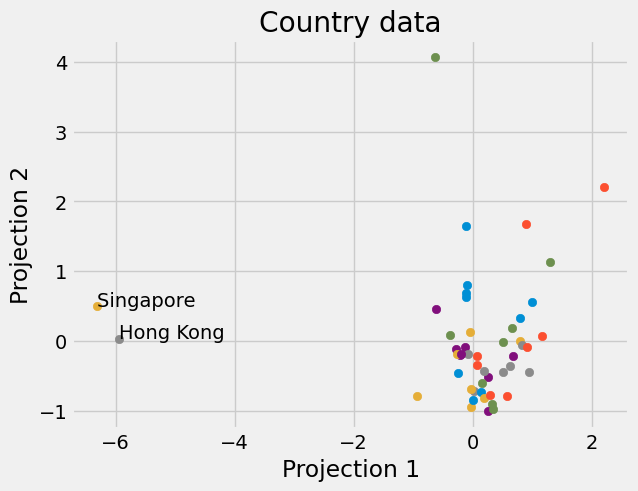
\includegraphics[width = 0.5\textwidth]{Images/problem 1b plot.png}
        \label{fig:problem 1b}
    \end{figure}

\begin{lstlisting}    
import pandas as pd
import numpy as np
import matplotlib.pyplot as plt

#filepaths for country data, names
filepathmat = 'datafiles/processed.txt'
filepathcont = 'datafiles/row.txt'
filepathdemvar = 'datafiles/column.txt'

#read in country names, then data with index as names
cont = pd.read_csv(filepathcont, header=None)
demvar = pd.read_csv(filepathdemvar, header=None)
df = pd.read_csv(filepathmat, header=None)
df = df.set_axis(cont[0], axis='index')

#Write to numpy array to do SVD
df_arr = df.to_numpy()
U, S, V = np.linalg.svd(df_arr)

testpts = []

j, k = 1, 2
for pts in range(U.shape[0]):
    testpts.append((S[j] *U[pts][j], S[k]*U[pts][k]))
pts = np.array(testpts)

#Finding outliers
outlier1 = np.argmin(pts[:, 0])
outpt1 = (outlier1, pts[outlier1, :])
outlier2 = np.argmin(np.delete(pts[:, 0], outlier1))
outpt2 = (outlier2, pts[outlier2, :])

outliers = np.array([df.index[outlier1], df.index[outlier2]])

for x, y in pts:
    plt.scatter(x, y)
    
plt.title("Country data")
plt.style.use('fivethirtyeight')
plt.gray
plt.ylabel(f'Projection {j}')
plt.xlabel(f'Projection {k}')
#Labelling outliers on plot
plt.annotate(f'{outliers[0]}', xy=(outpt1[1]) )
plt.annotate(f'{outliers[1]}', xy=(outpt2[1]) )
\end{lstlisting}
\end{solution}


\newpage
\subsection{Problem 1, part c}
Now do the same with the two left singular vectors of $A$, $\textbf{u}_1, \textbf{u}_2 \in \R^{49}$. Project the column vectors (i.e., variables) $\alpha_1, ..., \alpha_7 \in \R^{49}$ onto the two-dimensional space span$\{\textbf{u}_1, \textbf{u}_2\} \cong \R^2$ and plot this in a graph as before. Note that in this case, the points correspond to the demographic variables — label them accordingly.
\partbreak
\begin{solution}

The plot will be provided below, as well as the code. 

\begin{figure}[h]
    \centering
    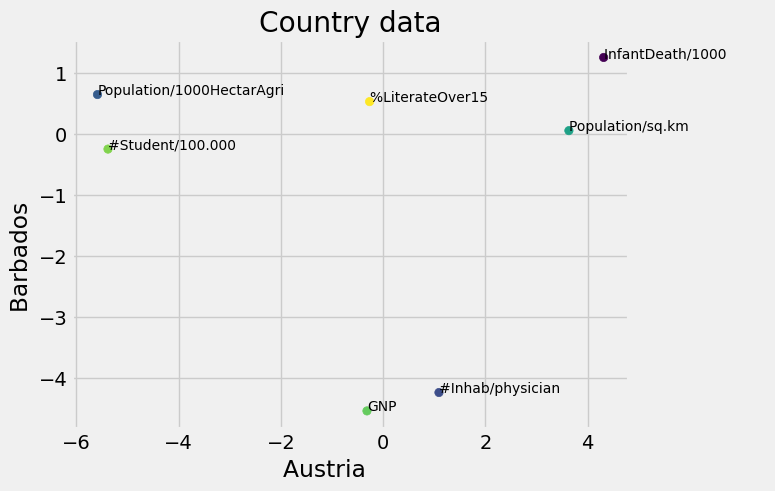
\includegraphics[width = 0.5\textwidth]{Images/problem 1c plot.png}
    \label{fig:problem1c}
\end{figure}

\begin{lstlisting}
#Doing the same except for demographic variables
testpts = []

j, k = 1, 2
for pts in range(V.shape[0]):
    testpts.append((S[j] *V[pts][j], S[k]*V[pts][k]))
pts = np.array(testpts)


# Create the scatter plot
plt.scatter(pts[:, 0], pts[:, 1], c = [random.randint(0, x*10) for x in range(len(V))])

#Finding outliers
for i, (x, y) in enumerate(pts):
    plt.annotate(f'{demvar[0][i]}', xy=(x, y), fontsize=10)

plt.title("Country data")
plt.style.use('fivethirtyeight')
plt.gray
plt.ylabel(f'{df.index[k]}')
plt.xlabel(f'{df.index[j]}')
\end{lstlisting}
\end{solution}

\newpage
\subsection{Problem 1, part d}
Overlay the two graphs in (b) and (c). Identify the two demographic variables near the two outlier countries — these explain why the two countries are outliers.
\partbreak
\begin{solution}

    Here is my plot. It seems like the two demographic variables very near to Singapore and Hong Kong are Population per 1000 Hectacr Agri and number of students per 100,000. These seem very reasonable, since these two countries are tightly packed, huge populations, and an emphasis on rigorous childhood education.

    \begin{figure}[h]
        \centering
        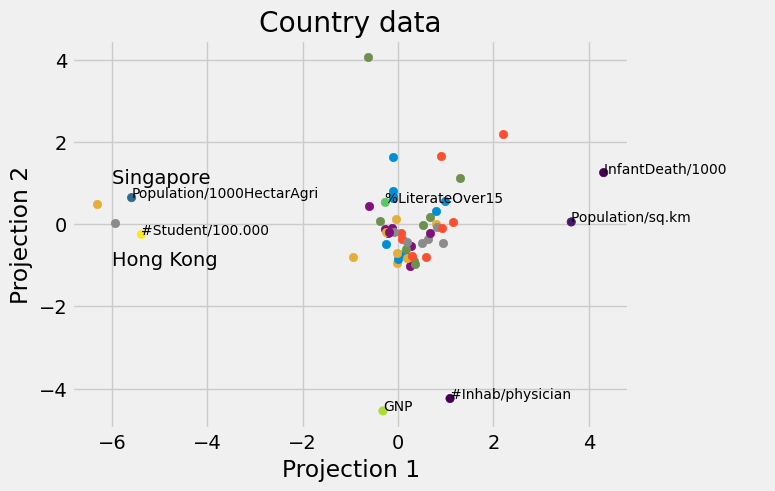
\includegraphics[width = 0.9\textwidth]{Images/biplot.png}
        \label{fig:p1c}
    \end{figure}
\end{solution}

\newpage
\subsection{Problem 1, part e}
Remove the two outlier countries and redo (b) with this 47 × 7 matrix. This allows you to see features that were earlier obscured by the outliers. Which two European countries are most alike Japan?
\partbreak
\begin{solution}
    Since you can't see the name too well on the map, I made some code to find the first few countries nearest to japan. Here's the code, then the plot. It seems that Portugal and Austria are most like japan in these projections (that are in Europe!).

    \begin{lstlisting}
dist = np.array([np.linalg.norm((x - pts[22][0], y - pts[22][1])) for x, y in pts])
k = 5
indices = np.argpartition(dist, k)[:k]

# Get the 3 minimum values and their indices
min_values = dist[indices]

print("Closest countries to Japan:",  df.index[indices])

Closest countries to Japan: Index(['Portugal      ', 'Japan         ', 'Austria       ', 'Mexico        ',
       'Costa Rica    '],
      dtype='object', name=0)
    \end{lstlisting}

    \begin{figure}[h]
        \centering
        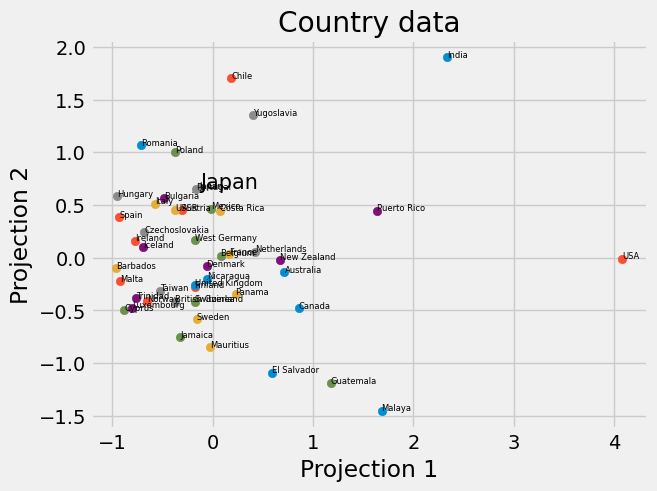
\includegraphics[width = 0.8\textwidth]{Images/japan.png}
        \label{fig:p1e}
    \end{figure}
\end{solution}
\newpage
\section{Problem 2}
Let $A, B \in \R^{m \times n}$ where $A$ has full column rank.

\subsection{Problem 2, part a}
Show that 
\[
\min_{X \in \R^{n\times m}} \norm{AX - \id_m}_F
\]
has a unique solution. What is the minimum length solution, i.e., where $\norm{X}_F$ is minimum?
\partbreak
\begin{solution}

    Suppose false, that is, there exists $X, X' \in \R^{n \times m}$ with $X \neq X'$ that achieve minimum. Then, via SVD, we can deduce a contradiction. Note the norm we are working with is the Frobenius norm, i will omit this in writing. We can also write $\id_m = UU^T$.
\newpage
{\small
    \alignbreak
    \begin{align}
        \norm{AX' - \id_m} &= \norm{AX - \id_m} &\text{(Both in argmin.)}\nonumber\\
        \norm{U\si V^t X' - UU^T} &= \norm{U\si V^t X - UU^T} &\text{(SVD of $A$.)}\nonumber\\
        \norm{\si V^TX' - U^T} &= \norm{\si V^TX - U^T} &\text{(Unitary invariance.)}\nonumber\\
        \tr \Big[ (\si V^TX' - U^T)^T(\si V^TX' - U^T)\Big] &= \tr \Big[ (\si V^TX' - U^T)^T(\si V^TX' - U^T)\Big] &\text{(Frobenius trace.)}\nonumber\\
        \tr \Big[ (\si V^TX')^T\si V^TX' - (\si V^TX'&)^TU^T - U\si V^TX' + UU^T\Big] =\\
        \tr \Big[ (\si V^TX)^T\si V^TX - (\si V^TX'&)^TU^T - U\si V^TX + UU^T\Big]\\
        1): \tr \Big[ X'^TV\si \si V^TX' - X'^TV\si U^T& - U\si V^TX' + UU^T\Big] &\text{(By symmetry 1 = 2.)}\nonumber\\
        \tr \Big[ X'^TV\si \si V^TX'\Big] - \tr \Big[ X'^TV\si U^T& \Big]- \tr \Big[ U\si V^TX'\Big] + \tr \Big[UU^T\Big] &\text{(Trace is linear.)}\nonumber\\
        \tr \Big[ X'^TV\si \si V^TX'\Big] - \tr \Big[ X'^TA^\dag& \Big]- \tr \Big[ AX'\Big] + \tr \Big[UU^T\Big] &\text{($A$ and $A\dag$.)}\nonumber\\
        \tr \Big[ V\si \si V^TX'X'^T\Big] - \tr \Big[ X'^TA^\dag& \Big]- \tr \Big[ AX'\Big] + \tr \Big[UU^T\Big] &\text{(Permutation in trace.)}\nonumber\\
        \tr \Big[ V\si \si V^T(X'X'^T - XX^T)\Big] + \tr \Big[& (X^T - X'^T)A^\dag \Big] + \tr \Big[ A(X - X')\Big] = 0 &\text{(Combining both.)}\nonumber\\
        \norm{V\si \si V^T(X'X'^T - XX^T)} + &\norm{(X^T - X'^T)A} + \norm{A(X - X')} = 0 &\text{(Frobenius definition.)}\nonumber\\
        \implies \norm{A(X - X')} = 0 &&\text{(All norms $\geq 0$, so all are 0.)}\nonumber\\
        \iff X - X' = 0 &&\text{(Norm definition.)}\nonumber\\
        \iff X = X'\nonumber
    \end{align}
    \alignbreak

}%
    Thus we found $X = X'$, which is a contradiction, so $X$ is unique. Aplologies for the bad formatting, this is the only way I could get it to fit.
\end{solution}

\newpage
\subsection{Problem 2, part b}
Show that the following method produces a symmetric matrix $X \in \R^{n \times n}$ that solves 
\[
\min_{X^T = X} \norm{AX - B}_F
\]
\subsubsection{i)}
show that the SVD of $A$ takes the form
\[
A = U\begin{bmatrix}\si \\ 0\end{bmatrix}V^T
\]
\partbreak
\begin{solution}

    We are given that $A$ is full column rank, thus full rank. Thus all singular values of $A > 0$. We then have two choices for $\si '$. Either $\si '$ is ``fat", where the zero matrix appears to the right of the singular values, or $\si'$ is ``skinny," meaning the zero matrix appear below. In either case, $\si'$ is $m \times n$, meaning it retains the same shape as $A$. Since $A$ is full \textit{column} rank, that means $\si'$ spans the entirety of $n$, so we are left with $\si'$ being the skinny case, which is the one shown.
\end{solution}
\subsubsection{ii)}
Show that 
\[
\norm{AX - B}_F^2 = \norm{\si Y - C_1}_F^2 + \norm{C_2}_F^2
\]
where $Y = V^TXV$ and $C = \begin{bmatrix}C_1\\C_2\end{bmatrix} = U^TBV$.
\partbreak
\begin{solution}

    We first note that the Frobenius norm is unitary invariant. That is, multiplying the argument inside by a unitary matrix does nothing to the result. If we multiply by $V$, the right eigenvectors of $A$, we get the following:
\newpage
    \alignbreak
    \begin{align}
        \norm{AX - B}_F^2 &= \norm{AXV - BV}_F^2 &\text{(Justified above.)}\nonumber\\
        &= \norm{U\si ' V^TXV - BV}_F^2 &\text{(SVD of $A$.)}\nonumber\\
        &= \tr \Big[ (U\si' Y - BV)^T(U\si' Y - BV) \Big] &\text{(Frobenius trace and $Y$ definition.)}\nonumber\\
        &= \tr \Big[ Y^T\si'^T U^TU\si 'Y - Y^T\si'^TU^TBV] &\text{(Distribution.)}\nonumber\\
        &= \tr \Big[ Y^T\si'^T\si^T Y - Y^T\si'^TC - C^T\si' Y + V^TB^TUU^TBV\Big] &\text{(Definition of $C$.)}\nonumber\\
        &= \tr \Big[ Y^T\si^T \si^T Y - Y^T\si ^TC_1 - C_1^T\si^TY + C^TC\Big] &\text{(Form of $\si'$ and $C$.)}\nonumber\\
        &= \tr \Big[ (\si Y)^T\si Y - (\si Y)^TC_1 - C_1^T \si Y + C_1^TC_1 + C_2^TC_2\Big] &\text{(Rewriting and form of $C$.)}\nonumber\\
        &= \tr \Big[ (\si Y - C_1)^T(\si Y - C_1)\Big] + \tr \Big[ C_2^TC_2\Big] &\text{(Trace is linear.)}\nonumber\\
        &=\norm{\si Y - C_1}_F^2 + \norm{C_2}_F^2 &\text{(Frobenius trace.)}\nonumber
    \end{align}
    \alignbreak
\end{solution}
\newpage
    \subsubsection{iii)}
    Note that $Y$ must be symmetric if $X$ is. Show that
    \[
    \norm{\si Y - C_1}_F^2 = \sum_{i = 1}^n |\si_iy_{ii} - c_{ii}|^2 + \sum_{j > i} (|\sigma_iy_{ij} - c_{ij}|^2 + |\sigma_jy_{ij} - c_{ji}|^2 
    \]

    and deduce that the minimum value above is attained when
    \[
    y_{ij} = \frac{\sigma_ic_{ij} + \sigma_jc_{ji}}{\sigma_i^2 + \sigma_j^2}
    \]
    for all $i, j = 1, ..., n$.
    \partbreak
    \begin{solution}

        This can be shown by the Frobenius norm and symmetry of $Y$.
{\small
        \alignbreak
        \begin{align}
            \norm{\si Y - C_1}_F^2 &= \sum_{i = 1}^n\sum_{j = 1}^n |\sigma_iy_{ij} - c_{ij}|^2 &\text{(Definition of Frobenius norm.)}\nonumber\\
            &= \sum_{i = 1}^n\Bigg[ \sum_{j = 1}^{i - 1} |\sigma_iy_{ij} - c_{ij}|^2 + |\sigma_iy_{ii} - c_{ii}|^2  + \sum_{j = i+1}^n |\sigma_iy_{ij} - c_{ij}|^2\Bigg] &\text{(Breaking $j$ sum up.)}\nonumber\\
            &= \sum_{i = 1}^n|\sigma_iy_{ii} - c_{ii}|^2 + \sum_{i = 1}^n\Bigg[ \sum_{j = 1}^{i - 1} |\sigma_iy_{ij} - c_{ij}|^2 + \sum_{j = i+1}^n |\sigma_iy_{ij} - c_{ij}|^2\Bigg]&\text{(Distribution.)}\nonumber\\
            &= \sum_{i = 1}^n|\sigma_iy_{ii} - c_{ii}|^2 + \sum_{i = 1}^n\Bigg[ \sum_{j = i+1}^{n} |\sigma_jy_{ji} - c_{ji}|^2 + \sum_{j = i+1}^n |\sigma_iy_{ij} - c_{ij}|^2\Bigg]&\text{(Transposition.)}\nonumber\\
            &= \sum_{i = 1}^n|\sigma_iy_{ii} - c_{ii}|^2 + \sum_{j > i}\Big[ |\sigma_jy_{ij} - c_{ji}|^2 + |\sigma_iy_{ij} - c_{ij}|^2\Big]&\text{(Symmetry of $Y$ and simplifying.)}\nonumber
        \end{align}
}%

\alignbreak
\newpage
We should expect the minimal symmetric $X$ to have only diagonal terms. Thus, we set the terms of the second sum to be equal zero. Thus, the following can be shown:

\alignbreak
\begin{align}
    0 &= (\sigma_jy_{ij} - c_{ji})^2 + (\sigma_iy_{ij} - c_{ij})^2 \nonumber\\
    &= \sigma_j^2 y_{ji}^2 + c_{ji}^2 - 2\sigma_jy_{ij}c_{ji} + \sigma_i^2y_{ij}^2 + c_{ij}^2 - 2\sigma_iy_{ij}c_{ij} &\text{(Expanding.)}\nonumber\\
    &= y_{ij}^2(\sigma^2_j + \sigma^2_i) - 2(\sigma_jc_{ji} + \sigma_ic_{ij})y_{ij} + (c_{ij}^2 + c_{ji}^2) &\text{(Grouping, polynomial in $y_{ij}$.)}\nonumber
\end{align}
\alignbreak

We can note that this polynomial is strictly positive, as this was how it was constructed. Then the minimum of the polynomial is at the vertex, $-b/2a$, meaning,

\[
y_{ij} = \frac{\sigma_jc_{ji} + \sigma_ic_{ij}}{\sigma_i^2 + \sigma_j^2}
\]

which is what we wanted to show. 
\end{solution}

\newpage
\section{Problem 2, part c}
Now emulate the previous part to find the rank-$r$ matrix $X \in \R^{m \times n}$ that solves 

\[
\min_{\text{rank}(X) \leq r}\norm{AX - B}_F.
\]

\partbreak
\begin{solution}

    Sorry, I did not have time this week to get to this part.
\end{solution}
\newpage
\section{Problem 3}
Let $A \in \C^{m\times n}$ and $\textbf{b} \in \C^m$. We will discuss a variant of $A\textbf{x} \approx \textbf{b}$ where the error occurs only in $A$. Note that in ordinary least squares we assume that the error occurs only in \textbf{b} while in total least squares we assume that it occurs in both $A$ and \textbf{b}.

\subsection{Problem 3, part a}
Show that if $0 \neq \textbf{x} \in \C^n$, then
\[
\norm{A\Big( \id - \frac{\textbf{x}\textbf{x}^*}{\textbf{x}^*\textbf{x}}\Big)}_F^2 = \norm{A}_F^2 - \frac{\norm{A\textbf{x}}_2^2}{\textbf{x}^*\textbf{x}}
\]
\partbreak
\begin{solution}

 Taking the left side, the following steps can be shown:

\vspace{-5mm}
 \alignbreak
 {\small
 \begin{align}
    \norm{A\Big( \id - \frac{\textbf{x}\textbf{x}^*}{\textbf{x}^*\textbf{x}}\Big)}^2_F &= \tr \Big[ \Big( A - \frac{1}{\textbf{x}^*\textbf{x}}A\textbf{x}\textbf{x}^*\Big)^*\Big( A - \frac{1}{\textbf{x}^*\textbf{x}}A\textbf{x}\textbf{x}^*\Big)\Big] &\text{(Frobenius trace.)}\nonumber\\
    &= \tr \Big[ A^*A\Big] - \frac{1}{\textbf{x}^*\textbf{x}} \tr \Big[ A^*A\textbf{x}\textbf{x}^*\Big] - \frac{1}{\textbf{x}^*\textbf{x}} \tr \Big[ (A\textbf{x}\textbf{x}^*)^*A\Big] + \frac{1}{(\textbf{x}^*\textbf{x})^2}\tr\Big[ (A\textbf{x}\textbf{x}^*)^*A\textbf{x}\textbf{x}^* \Big] &\text{(Expanding.)}\nonumber\\
    &= \norm{A}_F^2 - \frac{1}{\textbf{x}^*\textbf{x}} \tr \Big[ A^*A\textbf{x}\textbf{x}^*\Big] - \frac{1}{\textbf{x}^*\textbf{x}} \tr \Big[ \textbf{x}\textbf{x}^*A^*A\Big] + \frac{1}{(\textbf{x}^*\textbf{x})^2}\tr\Big[ \textbf{x}\textbf{x}^*A^*A\textbf{x}\textbf{x}^* \Big] &\text{(Hermiting(?).)}\nonumber\\
    &= \norm{A}_F^2 - \frac{1}{\textbf{x}^*\textbf{x}} \tr \Big[ \textbf{x}^*A^*A\textbf{x}\Big] - \frac{1}{\textbf{x}^*\textbf{x}} \tr \Big[ \textbf{x}^*A^*A\textbf{x}\Big] + \frac{1}{(\textbf{x}^*\textbf{x})^2}\tr\Big[ A^*A\textbf{x}\textbf{x}^* \textbf{x}\textbf{x}^*\Big] &\text{(Trace permutating.)}\nonumber\\
    &= \norm{A}_F^2 - \frac{1}{\textbf{x}^*\textbf{x}} \tr \Big[ (A\textbf{x})^*A\textbf{x}\Big] - \frac{1}{\textbf{x}^*\textbf{x}} \tr \Big[ (A\textbf{x})^*A\textbf{x}\Big] + \frac{1}{(\textbf{x}^*\textbf{x})^2}\tr\Big[ A^*A\textbf{x}(\textbf{x}^* \textbf{x})\textbf{x}^*\Big] &\text{(Hermiting, associating.)}\nonumber\\
    &= \norm{A}_F^2 - \frac{1}{\textbf{x}^*\textbf{x}} \norm{A\textbf{x}}_2^2 - \frac{1}{\textbf{x}^*\textbf{x}} \norm{A\textbf{x}}_2^2 + \frac{1}{\textbf{x}^*\textbf{x}}\tr\Big[ A^*A\textbf{x}\textbf{x}^*\Big] &\text{(Trace of scalar is scalar.)}\nonumber\\
     &= \norm{A}_F^2 - \frac{1}{\textbf{x}^*\textbf{x}} \norm{A\textbf{x}}_2^2 - \frac{1}{\textbf{x}^*\textbf{x}} \norm{A\textbf{x}}_2^2 + \frac{1}{\textbf{x}^*\textbf{x}}\tr\Big[ \textbf{x}^*A^*A\textbf{x}\Big] &\text{(Permutating.)}\nonumber\\
     &= \norm{A}_F^2 - \frac{1}{\textbf{x}^*\textbf{x}} \norm{A\textbf{x}}_2^2 - \frac{1}{\textbf{x}^*\textbf{x}} \norm{A\textbf{x}}_2^2 + \frac{1}{\textbf{x}^*\textbf{x}}\norm{A\textbf{x}}_2^2 &\text{(Trace of scalar is scalar.)}\nonumber\\
     &=\norm{A}_F^2 - \frac{\norm{A\textbf{x}}_2^2}{\textbf{x}^*\textbf{x}} &\text{(Simplifying.)}\nonumber
 \end{align}
 }%
 \alignbreak

\end{solution}

\newpage
\subsection{Problem 3, part b}
Show that the matrix 
\[
E = \frac{(\textbf{b} - A\textbf{x})\textbf{x}^*}{\textbf{x}^*\textbf{x}} \in \C^{m\times n}
\]
has the smallest 2-norm among all $E \in \C^{m\times n}$ that satisfy 
\[
(A + E) \textbf{x} = \textbf{b}
\]
\partbreak
\begin{solution}

 Note that all $E$'s satisfy $E\textbf{x} = \textbf{b} - A\textbf{x}$. To distinguish the $E$ matrices, we'll denote $E'$ as a matrix that satisfies $(A+E')\textbf{x} = \textbf{b}$. Thus, the following can be shown:

 \alignbreak
 \begin{align}
     \norm{E}_2^2 &= \norm{\frac{(\textbf{b} - A\textbf{x})\textbf{x}^*}{\textbf{x}^*\textbf{x}}}^2_2 &\text{(Given.)}\nonumber\\
     &= \Big| \frac{1}{\textbf{x}^*\textbf{x}}\Big|^2 \norm{(\textbf{b} - A\textbf{x})\textbf{x}^*}_2^2 &\text{(Denominator is real.)}\nonumber\\
     &\leq \Big| \frac{1}{\textbf{x}^*\textbf{x}}\Big|^2 \norm{\textbf{b} - A\textbf{x}}_2^2\norm{\textbf{x}^*}_2^2 &\text{(Cauchy Schwartz.)}\nonumber\\
     &= \frac{\norm{\textbf{b} - A\textbf{x}}_2^2}{\norm{\textbf{x}}^2_2} &\text{(Simplifying.)}\nonumber\\
     &= \frac{\norm{E'\textbf{x}}_2^2}{\norm{\textbf{x}}_2^2} &\text{(Equality above.)}\nonumber\\
     &\leq \norm{E'}_2^2 \frac{\norm{\textbf{x}}_2^2}{\norm{\textbf{x}}_2^2} &\text{(Consistency of 2-norm.)}\nonumber\\
     \implies \norm{E}_2^2&\leq \norm{E'}_2^2 &\text{(Simplifying.)}\nonumber\\
     \iff \norm{E}_2 &\leq \norm{E'}_2 \nonumber
 \end{align}
 \alignbreak
\end{solution}

\newpage
\subsection{Problem 3, part c}
Let $A, \textbf{b}, \textbf{x}$ be given and fixed. What are the solutions of 
\[
    \min_{(A+E)\textbf{x} = \textbf{b}} \norm{E}_2 \hspace{3mm} \text{and} \hspace{3mm} \min_{(A+E)\textbf{x} = \textbf{b}} \norm{E}_F
\]
where the minimum is taken over all $E \in \C^{m\times n}$ such that $(A+E)\textbf{x} = \textbf{b}$?
\partbreak
\begin{solution}

We just showed in the previous part that when 
\[
    E = \frac{(\textbf{b} - A\textbf{x})\textbf{x}^*}{\textbf{x}^*\textbf{x}} \in \C^{m\times n}
\] 

 Then $E$ is the smallest of all $E$'s satisfying $(A+E)\textbf{x} = \textbf{b}$. We can then just plug this value for $E$ in to get the minimum value for each.

 \alignbreak
 \begin{align}
     \min_{(A+E)\textbf{x} = \textbf{b}} \norm{E}_2 &= \norm{\frac{(\textbf{b} - A\textbf{x})\textbf{x}^*}{\textbf{x}^*\textbf{x}}}_2 &\text{(Plugging in.)}\nonumber\\
     &= \frac{1}{\norm{\textbf{x}}_2^2}\norm{\textbf{b}\textbf{x}^* - A\textbf{x}\textbf{x}^*}_2 &\text{(Simplifying.)}\nonumber\\
     \min_{(A+E)\textbf{x} = \textbf{b}} \norm{E}_F &= \frac{1}{\norm{\textbf{x}}_2^2}\tr\Big[ (\textbf{b}\textbf{x}^* - A\textbf{x}\textbf{x}^*)^*(\textbf{b}\textbf{x}^* - A\textbf{x}\textbf{x}^*)\Big] &\text{(Frobenius trace.)}\nonumber\\
     &= \frac{1}{\norm{\textbf{x}}_2^2}\tr\Big[ \textbf{x}\textbf{b}^*\textbf{b}\textbf{x}^* + \textbf{x}\textbf{x}^*A^*A\textbf{x}\textbf{x}^* - \textbf{x}\textbf{b}^*A\textbf{x}\textbf{x}^* - \textbf{x}\textbf{x}^*A^*\textbf{b}\textbf{x}^*\Big] &\text{(Hermiting.)}\nonumber\\
     &= \frac{1}{\norm{\textbf{x}}_2^2}\tr\Big[ \norm{\textbf{b}}_2^2\textbf{x}\textbf{x}^* + A^*A\textbf{x}\textbf{x}^*\textbf{x}\textbf{x}^* - \textbf{b}^*A\textbf{x}\textbf{x}^*\textbf{x} - \textbf{x}^*A^*\textbf{b}\textbf{x}^*\textbf{x}\Big] &\text{(Permuting.)}\nonumber\\
     &= \frac{1}{\norm{\textbf{x}}_2^2}\tr\Big[ \norm{\textbf{b}}_2^2\norm{\textbf{x}}_2^2 + \norm{\textbf{x}}_2^2\norm{A\textbf{x}}_2^2 - \norm{\textbf{x}}_2^2\textbf{b}^*A\textbf{x} - \norm{\textbf{x}}_2^2\textbf{x}^*A^*\textbf{b}\Big] &\text{(Taking norms.)}\nonumber\\
     &= \tr\Big[ \norm{\textbf{b}}_2^2 + \norm{A\textbf{x}}_2^2 - \textbf{b}^*A\textbf{x} - \textbf{x}^*A^*\textbf{b}\Big] &\text{(Simplifying.)}\nonumber\\
     &= \norm{\textbf{b}}_2^2 + \norm{A\textbf{x}}_2^2 - 2\tr \Big[ \textbf{b}^*A\textbf{x}\Big] &\text{(Simplifying.)}\nonumber
 \end{align}
 \alignbreak
\end{solution}

\newpage
\subsection{Problem 3, part d}
Given $\textbf{a} \in \C^n, \textbf{b} \in \C^m$, and $\delta > 0$. Show how to solve the problems 
\[
\min_{\norm{E}_F \leq \delta} \norm{E\textbf{a} - \textbf{b}}_2 \hspace{5mm} \text{and} \hspace{5mm} \max_{\norm{E}_F \leq \delta} \norm{E\textbf{a} - \textbf{b}}_2
\]
\partbreak
\begin{solution}

    Sorry, I didn't get to this part in time, but I will try to explain my thoughts. I would imagine you would want $E$ to map $\textbf{a}$ the closest to $\textbf{b}$ in the minimize problem, but $E$ can only stretch $\textbf{a}$ at most size $\delta$. If The distance from $\textbf{a}$ to $\textbf{b}$ is less than $\delta$, then the minimum can be achieved for some $E$, so our minimum value would be 0. If not, then you would just take the distance from zero to the origin. If this distance is smaller than the distance to $\textbf{b}$, then just let $E = 0$. \par

    \vspace{5mm}
    For the maximizer, you would just want $E$ to map $\textbf{a}$ the furthest away from $\textbf{b}$. If $\textbf{a}$ is greater than $\textbf{b}$ by distance $\delta$, then you would just map it further away. 
\end{solution}
\newpage
\section{Problem 4}
In the following, $\kappa(A) := \norm{A}\norm{A^\dag}$ for $A\in \C^{m\times n}$ where $\norm{\cdot}$ denotes a submultiplicative matrix norm. We will write $\kappa_p(A)$ if the norm involved is a matrix p-norm. 

\subsection{Problem 4, part a}
Show that for any nonzero $A \in \C^{m\times n}$, $\kappa(A) \geq 1$.

\partbreak
\begin{solution}

 We are given that $\norm{\cdot}$ is submultiplicative, thus $\norm{A}\norm{A^\dag} \geq \norm{AA^\dag}.$ If A is invertible, then $AA^\dag = AA^{-1} = \id$. Note that $\norm{\id} = \norm{\id^2} \leq \norm{\id}^2$, thus $\norm{\id} \geq 1$ for any submultiplicative norm. Then $\kappa(A) = \norm{A}\norm{A^\dag} \geq 1$. If $A$ is not invertible, then we can use SVD. We will write $A = U\Sigma V^*$, so $A^\dag = V\Sigma^\dag U^*$. Then,

 \alignbreak
 \begin{align}
     \norm{AA^\dag} &= \norm{U\Si V^* V \Si ^\dag U^*} &\text{(By SVD.)}\nonumber\\
     &= \norm{U\Si\Si ^\dag U^*} &\text{($V$ is hermitian.)}\nonumber\\
     &= \norm{U\begin{bmatrix}\id_r\\0\end{bmatrix}U^*}, \norm{U\begin{bmatrix}\id_r &0\end{bmatrix}U*} &\text{(Depends if $m \geq n$, or reverse.)}\nonumber\\
     &= \norm{U_rU^*} &\text{(In either case, we take the first r vectors of $U$.)}\nonumber\\
     &= \norm{\id_r} &\text{(Simplifying.)}\nonumber\\
     &\geq 1 &\text{(Identity is $\geq 1$.)}\nonumber
 \end{align}
 \alignbreak

 Note in these steps, I took the first $r$ rows \textit{or} columns from $U$ or $U^*$. Without loss of generality, since $U$ is hermitian, the above is given. Note that $\id_r$ in the last step is an $m \times n$ matrix, which I take its norm as in the $r\times r$ case. 
\end{solution}

\newpage
\subsection{Problem 4, part b}
Show that for any $A \in \C^{m\times n}$,
\[
    \kappa_2(A^*A) = \kappa_2(A)^2
\]
but that in general,
\[
    \kappa(A^*A)\neq \kappa(A)^2
\]
\partbreak
\begin{solution}

We know that $A^*A$ will have eigenvalues $|\lm|^2$ for eigenvalue $\lm$ of A. Thus, $\norm{A^*A}_2 = \max \{ |\lm|\} = (\max \{ |\lm | \})^2$. Similarly, $(A^*A)^{-1}$ has eigenvalues $1/|\lm|^2$. Note that $A^*A$ is positive \textit{semi}-definite, so any eigenvalue of $A^*A$ is $\geq 0$. If there is an eigenvalue equal zero, then $\kappa_2(A^*A) = \infty$. This also happens for $\kappa(A)$, since $\max \{ 1/|\lm|\} = \infty$. If we still take the SVD of $A^*A$, just to be safe, then 
\[
\kappa_2(A^*A) = \norm{A^*A}_2\norm{(A^*A)^{-1}}_2 = \frac{(\max{|\lm|})^2}{(\max{1/|\sigma^2|})} = (\max{|\lm|})^2 (\min{|\sigma|})^2
\]
Here we cannot assume that $A$ is invertible, but by SVD, we can say what the 2-norm of $A^{-1}$ is. This will then be the largest singular value of $\si ^\dag$, which is the smallest singular value of $\si$. Thus when squaring, we get
\[
\kappa_2(A)^2 = (\norm{A}_2\norm{A^\dag}_2)^2 = (\max\{|\lm|\})^2(\min \{ \sigma \} )^2
\]

Thus, these two are equivalent. This should hold true for any norm, by the equivalence of norms over a finite dimensional vector space.  
\end{solution}

\newpage
\subsection{Problem 4, part c}
Show that for nonsingular $A, B \in \C^{n\times n}$, 
\[
\kappa(AB)\leq \kappa(A)\kappa(B).
\]
 It this true in general without the nonsingular condition?
 \partbreak
 \begin{solution}

     For nonsingular $A, B$, this property is easy to show. Note the pseudoinverse turns into a normal inverse for the product.

     \alignbreak
     \begin{align}
         \kappa(AB) &= \norm{AB}\norm{(AB)^{-1}} &\text{(Given.)}\nonumber\\
         &= \norm{AB} \norm{B^{-1}A^{-1}} &\text{(Inverse of $AB$.)}\nonumber\\
         &\leq \norm{A} \norm{B} \norm{B^{-1}} \norm{A^{-1}} &\text{(Submultiplication.)}\nonumber\\
         \implies \kappa(AB) &\leq \kappa(A)\kappa(B)\nonumber
     \end{align}
     \alignbreak
 \end{solution}

\newpage
 \subsection{Problem 4, part d}
 Let $Q \in \C^{n\times n}$ be a matrix with orthonormal columns. Show that 
 \[
 \kappa_2(Q) = 1.
 \]
 Is this true if $Q$ has orthonormal rows instead? Is this true with $\kappa_1$ or $\kappa_\infty$ in place of $\kappa_2$?
 \partbreak
 \begin{solution}
     First, note that the 2-norm is unitary invariant, Since $Q^* = Q^{-1}$, then 
     \[
     \kappa_2(Q) = \norm{Q}_2 \norm{Q^{-1}}_2 = \norm{Q}_2\norm{Q^T}_2 = \norm{\id}_2\norm{\id}_2 = 1
     \]

     I wrote the above equality to emphasize that this will work is $Q$ has orthonormal rows instead, since the $Q$ and $Q^T$ terms will just swap around. Since $\kappa_1$ is taken with the one matrix norm, it will take the max absolute row sum of $Q$, which is 1 since $Q$ has orthonormal columns. This is the same for $\kappa_\infty$, as again the $Q$ and $Q^T$ terms will just swap.  
 \end{solution}

 \subsection{Problem 4, part e}
 Let $R \in \C^{n\times n}$ be a nonsingular upper-triangular matrix. Show that
 \[
 \kappa_\infty(R) \geq \frac{\max_{i = 1, ..., n}|r_{ii}|}{\min_{i = 1, ..., n}|r_{ii}|}
 \]
 \partbreak
 Note for an upper triangular matrix, its eigenvalues are on the diagonal, so we can note the numerator of the right hand side is just $\norm{R}_2$. If we can accept that the diagonal of the inverse of $R$ is just the inverted diagonal of $R$, then 
 \[
 \min |r_{ii}| = \max 1/|r_{ii}| = \max 1/|\lm_i| = \norm{R^{-1}}_2
 \]

 That is, since the upper triangular matrices form a closed subgroup of $GL(n)$, then we can say the diagonal or $R^{-1}$ is the inverse of the diagonal of $R$. We already know that $R^{-1}$ will have eigenvaules $1/\lm_i$ for $\lm_i$ of $R$. They are all nonzero, so this is valid. So the right hand side is just $\kappa_2(R)$. We just need to show that 
 \[
 \kappa_\infty(R) \geq \kappa_2(R).
 \]
 By the equivalence of norms, $\norm{R}_2 \leq \sqrt{n}\norm{R}_\infty$ for any positive $n$, so $\norm{R}_2 \leq \norm{R}_\infty$. This argument also holds for $R^{-1}$. Thus, $\kappa_2(R) \leq \kappa_\infty(R)$. 

\newpage
 \subsection{Problem 4, part f}
 Show that for any nonsingular $A \in \C^{n\times n}$, 
 \[
 \kappa(A) \leq \max \Bigg\{ \frac{\norm{AX - \id}}{\norm{XA - \id}}, \frac{\norm{XA - \id}}{\norm{AX - \id}} \Bigg\}
 \]
 \partbreak
 \begin{solution}

     We are given $\norm{\cdot}$ is submultiplicative, so we can note, by the hint, that
     \[
     \norm{AX - \id} = \norm{A(XA - \id)A^{-1}} \leq \norm{A} \norm{XA- \id} \norm{A^{-1}}
     \]
     By rearranging, we get 
     \[
     \frac{\norm{AX - \id}}{\norm{XA - \id}} \leq \norm{A}\norm{A^{-1}} = \kappa(A)
     \]

     This shows the first inequality. Next note that we could have also don't the same for $XA - \id$, that is, $A^{-1}(AX - \id) A = XA - \id$. We can then write the following

     \[
     \norm{XA - \id} = \norm{A^{-1}(AX - \id) A} \leq \norm{A^{-1}}\norm{AX - \id}\norm{A}.
     \]

     Which can then be rewritten as 
     \[
     \frac{\norm{XA - \id}}{\norm{AX - \id}} \leq \norm{A^{-1}} \norm{A} = \kappa(A),
     \]

     thus the second inequality has been shown, so $\kappa(A)$ is greater than both, so it is greater than the max. 
 \end{solution}
\newpage
\section{Problem 5}
We will examine the effect of various parameters on the accuracy of a computed solution to a nonsingular linear system. Relevant commands in Matlab syntax are given in brackets.

\subsection{Problem 5, part a}
Generate $A = [a_{ij}] \in \R^{n\times n}$ as follows:
\begin{enumerate}
    \item $a_{ij}$ randomly generated from a standard normal distribution $[randn(n)]$. 
    \item A Hilbert matrix, i.e. $a_{ij} = 1/(i + j - 1)$
    \item A Pascal matrix
    \item A magic square
\end{enumerate}
\partbreak
\begin{solution}
    I will provide my definitions below. Note that I had some external help creating the magic square.

    \begin{lstlisting}
import numpy as np
import random
import math
def random_matrix(n: int):
    """
    Returns a numpy matrix of size n by n filled with random numbers 
    """
    res = np.zeros((n, n))
    for i in range(res.shape[0]):
        for j in range(res.shape[1]):
            res[i][j] = random.gauss(0, 1)
    return res

def hilbert_matrix(n: int):
    """
    Returns a Hilbert matrix of size n by n where 
    a_{ij} = 1/ (i + j - 1)
    """
    res = np.zeros((n , n))
    for i in range(n):
        for j in range(n):
            if i== 0 and j ==0:
                res[i][j] = 1
            else:
                res[i][j] = float(1 / ((i+1) + (j+1) - 1))
    return res

def pascal_matrix(n: int):
    """
    Returns a Pascal matrix of size n with entries 
    a_{ij} = {i + j \choose i}
    """
    res = np.zeros((n, n))
    for i in range(n):
        for j in range(n):
            res[i][j] = math.comb(i+j, i)
    return res

def magic_matrix(N: int):
    """
    Returns a magic square of size N by N. 
    Courtesy of https://scipython.com/book/chapter-6-numpy/examples/creating-a-magic-square/
    """

    magic_square = np.zeros((N,N), dtype=int)

    n = 1
    i, j = 0, N//2

    while n <= N**2:
        magic_square[i, j] = n
        n += 1
        newi, newj = (i-1) % N, (j+1)% N
        if magic_square[newi, newj]:
            i += 1
        else:
            i, j = newi, newj
    
    return magic_square
    \end{lstlisting}
\end{solution}
\newpage
\subsection{Problem 5, part b}
Generate $\textbf{x}$ and $\textbf{b} \in \R^n$ as follows:
\begin{enumerate}
    \item $\textbf{x} = [1, ..., 1]^T$
    \item $\textbf{b} = A\textbf{x}$
\end{enumerate}
\partbreak
\begin{solution}
    
    Here is my code:
    \begin{lstlisting}
def one_vect(n: int):
    """
    Returns a column vector of size n x 1 filled with ones 
    """
    return np.ones((n, 1))

def mat_vec_mult(A: np.ndarray, x: np.array):
    """
    Returns the multiplication of Ax. Has no protection on it
    so be careful.
    """
    return np.matmul(A, x)
    \end{lstlisting}
\end{solution}
\newpage
\subsection{Problem 5, part c}
 For each A generated as above, perform the following for $n = 5, 10, 15, . . . , 500$.
 \begin{enumerate}
     \item Solve $A\textbf{x} = \textbf{b}$  using your program to get $\hat{\textbf{x}}$. Note that in general the result computed by your program will not exactly be the true solution $\textbf{x} = A^{-1}\textbf{b}$ because of roundoff errors that occurred during computations.
 
    \item Compute $\Delta b = A\hat{\textbf{x}} - \textbf{b}$ and record the values of $\norm{\textbf{x} - \hat{\textbf{x}}}/ \norm{\textbf{x}}, \kappa(A) and \kappa(A)\norm{\Delta \textbf{b}} / \norm{\textbf{b}}$ for $\norm{\cdot} = \norm{\cdot}_1, \norm{\cdot}_2, \norm{\cdot}_\infty$

    \item Present everything for the $n = 5$ case but only tabulate the relevant trend for general $n > 5 in a graph.$
 \end{enumerate}
\partbreak
 \begin{solution}
     Here is my code (don't judge me, I only had like 2 days to work on this homework)

     \begin{lstlisting}
xhats = []
deltab = []

#x - xhat / mag x
xmag1 = []
xmag2 = []
xmaginf = []

#cond numbers
con1 = []
con2 = []
coninf = []

#max b * cond
relcon1 = []
relcon2 = []
relconinf = []

for inc in range(5, 505, 5):
    vec = one_vect(inc)
    ran = random_matrix(inc)
    hil = hilbert_matrix(inc)
    pas = pascal_matrix(inc)
    mag = magic_matrix(inc)
    
    ransol = np.matmul(np.linalg.pinv(ran), vec)
    hilsol = np.matmul(np.linalg.pinv(hil), vec)
    passol = np.matmul(np.linalg.pinv(pas), vec)
    magsol = np.matmul(np.linalg.pinv(mag), vec)
    
    dbran = np.matmul(ran, ransol) - mat_vec_mult(ran, vec) 
    dbhil = np.matmul(hil, hilsol) - mat_vec_mult(hil, vec)
    dbpas = np.matmul(pas, passol) - mat_vec_mult(pas, vec)
    dbmag = np.matmul(mag, magsol) - mat_vec_mult(mag, vec)
    
    magran1 = np.linalg.norm(vec - ransol, ord= 1) / np.linalg.norm(vec, ord = 1)
    maghil1 = np.linalg.norm(vec - hilsol, ord= 1) / np.linalg.norm(vec, ord = 1)
    magpas1 = np.linalg.norm(vec - passol, ord= 1) / np.linalg.norm(vec, ord = 1)
    magmag1 = np.linalg.norm(vec - magsol, ord= 1) / np.linalg.norm(vec, ord = 1)
    
    
    magran2 = np.linalg.norm(vec - ransol, ord= 2) / np.linalg.norm(vec, ord = 2)
    maghil2 = np.linalg.norm(vec - hilsol, ord= 2) / np.linalg.norm(vec, ord = 2)
    magpas2 = np.linalg.norm(vec - passol, ord= 2) / np.linalg.norm(vec, ord = 2)
    magmag2 = np.linalg.norm(vec - magsol, ord= 2) / np.linalg.norm(vec, ord = 2)
    
    
    magraninf = np.linalg.norm(vec - ransol, ord= np.inf) / np.linalg.norm(vec, ord = np.inf)
    maghilinf = np.linalg.norm(vec - hilsol, ord= np.inf) / np.linalg.norm(vec, ord = np.inf)
    magpasinf = np.linalg.norm(vec - passol, ord= np.inf) / np.linalg.norm(vec, ord = np.inf)
    magmaginf = np.linalg.norm(vec - magsol, ord= np.inf) / np.linalg.norm(vec, ord = np.inf)
    
    rancon1 = np.linalg.cond(ran, p=1)
    hilcon1 = np.linalg.cond(hil, p=1)
    pascon1 = np.linalg.cond(pas, p=1)
    magcon1 = np.linalg.cond(mag, p=1)

    rancon2 = np.linalg.cond(ran, p=2)
    hilcon2 = np.linalg.cond(hil, p=2)
    pascon2 = np.linalg.cond(pas, p=2)
    magcon2 = np.linalg.cond(mag, p=2)

    ranconinf = np.linalg.cond(ran, p=np.inf)
    hilconinf = np.linalg.cond(hil, p=np.inf)
    pasconinf = np.linalg.cond(pas, p=np.inf)
    magconinf = np.linalg.cond(mag, p=np.inf)
    
    relconran1 = rancon1 * np.linalg.norm(dbran, ord = 1) / np.linalg.norm(vec, ord = 1)
    relconhil1 = hilcon1 * np.linalg.norm(dbhil, ord = 1) / np.linalg.norm(vec, ord = 1)
    relconpas1 = pascon1 * np.linalg.norm(dbpas, ord = 1) / np.linalg.norm(vec, ord = 1)
    relconmag1 = magcon1 * np.linalg.norm(dbmag, ord = 1) / np.linalg.norm(vec, ord = 1)
    
    relconran2 = rancon2 * np.linalg.norm(dbran, ord = 2) / np.linalg.norm(vec, ord = 2)
    relconhil2 = hilcon2 * np.linalg.norm(dbhil, ord = 2) / np.linalg.norm(vec, ord = 2)
    relconpas2 = pascon2 * np.linalg.norm(dbpas, ord = 2) / np.linalg.norm(vec, ord = 2)
    relconmag2 = magcon2 * np.linalg.norm(dbmag, ord = 2) / np.linalg.norm(vec, ord = 2)
    
    relconraninf = ranconinf * np.linalg.norm(dbran, ord = np.inf) / np.linalg.norm(vec, ord = np.inf)
    relconhilinf = hilconinf * np.linalg.norm(dbhil, ord = np.inf) / np.linalg.norm(vec, ord = np.inf)
    relconpasinf = pasconinf * np.linalg.norm(dbpas, ord = np.inf) / np.linalg.norm(vec, ord = np.inf)
    relconmaginf = magconinf * np.linalg.norm(dbmag, ord = np.inf) / np.linalg.norm(vec, ord = np.inf)
    
    temp11 = [relconraninf, relconhilinf, relconpasinf, relconmaginf]
    temp10 = [relconran2, relconhil2, relconpas2, relconmag2]
    temp9 = [relconran1, relconhil1, relconpas1, relconmag1]
    temp8 = [ranconinf, hilconinf, pasconinf, magconinf]
    temp7 = [rancon2, hilcon2, pascon2, magcon2]
    temp6 = [rancon1, hilcon1, pascon1, magcon1]
    temp5 = [magran1, maghil1, magpas1, magmag1]
    temp4 = [magran2, maghil2, magpas2, magmag2]
    temp3 = [magraninf, maghilinf, magpasinf, magmaginf]
    temp2 = [dbran, dbhil, dbpas, dbmag]
    temp1 = [ransol, hilsol, passol, magsol]
    
    xhats.append(temp1)
    deltab.append(temp2)
    xmag1.append(temp5)
    xmag2.append(temp4)
    xmaginf.append(temp3)
    con1.append(temp6)
    con2.append(temp7)
    coninf.append(temp8)
    relcon1.append(temp9)
    relcon2.append(temp10)
    relconinf.append(temp11)
     \end{lstlisting}

 This disgusting abomination will record everything for us. Here is the $n = 5$ case wrapped in a numpy array:

 \begin{figure}[h]
     \centering
     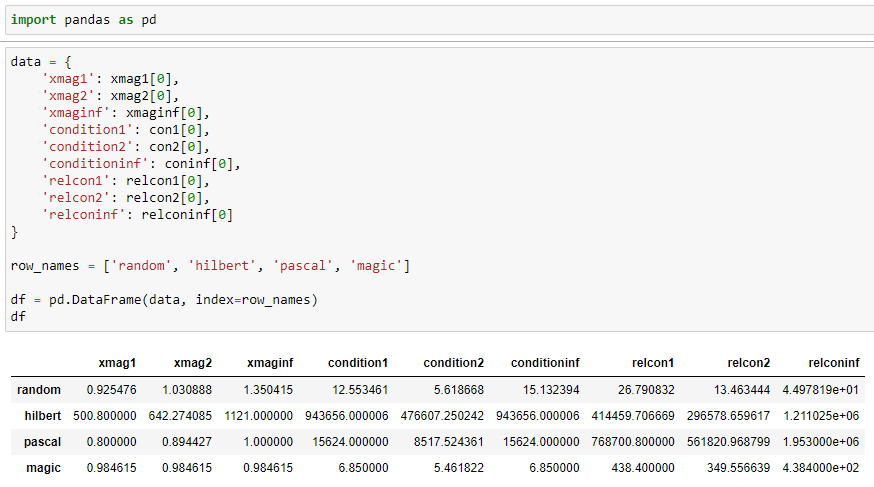
\includegraphics[width = \textwidth]{Images/dataframe.png}
     \label{p5c: dataframe}
 \end{figure}

 Here are the trends for the three different values to consider:

 \begin{figure}
     \centering
     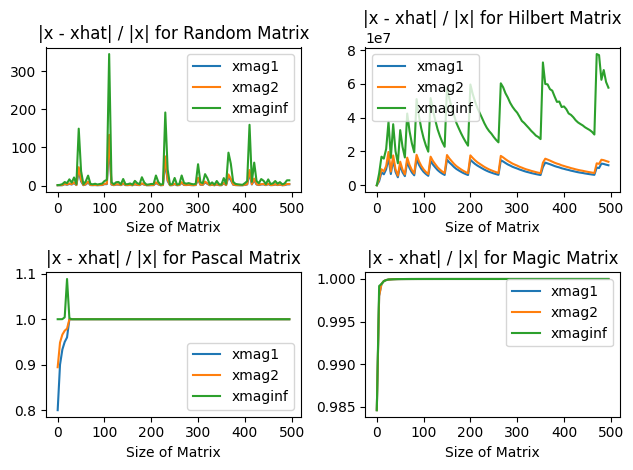
\includegraphics{Images/mags.png}
     \label{fig:xhats}
 \end{figure}

 \begin{figure}
     \centering
     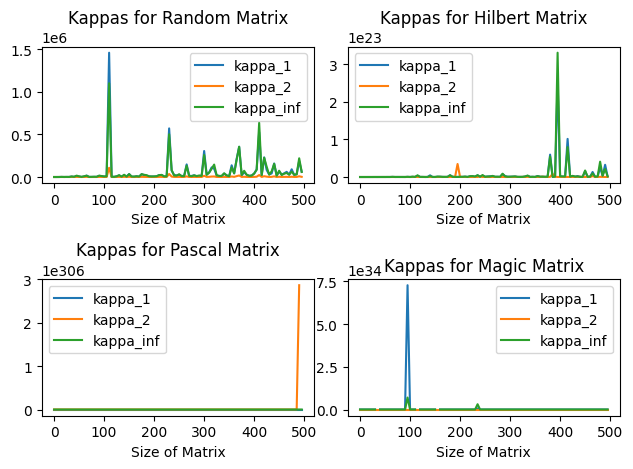
\includegraphics{Images/kappas.png}
     \label{fig:relcon}
 \end{figure}

 \begin{figure}
     \centering
     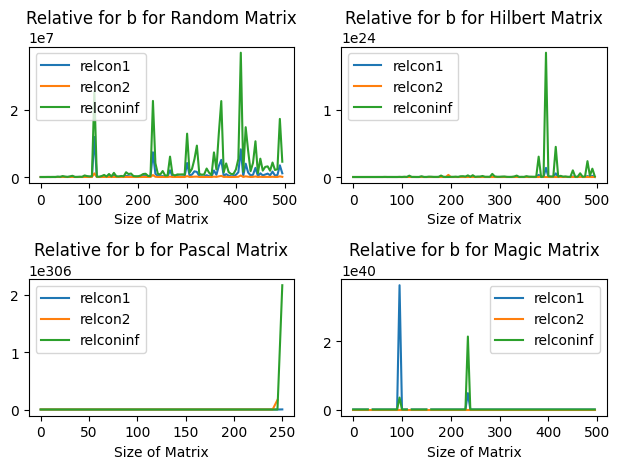
\includegraphics{Images/relb.png}
     \label{fig:relmags}
 \end{figure}
 \end{solution}

\newpage
\subsection{Problem 5, part d}
Discuss an explain the effects of different choices of $A$, $b$, $\norm{\cdot}$, and $n$ have on the accuracy of the computed solution $\hat{\textbf{x}}$.
\partbreak
\begin{solution}

    For the relative magnitudes for $x_hat$, we see wildly different plots for the random matrix, the Hilbert matrix, and Pascal Matrix. It looks like the Magic matrix has nearly the same shape as the pascal matrix. There seems to be some periodicity in the Hilbert matrix, and the relative magnitude difference is quite massive compared to other plots. It also seems that the mags stayed relatively the same shape for each matrix, aside from the Hilbert matrix.\par 

    For the condition number of these matrices, they seem relatively stable, aside from a few rogue points on the plot. Admittedly, I probably should have removed these points to get a far more interesting plot. \par

    It seems as though the relative b suffered the same problem as the conditional number plots. The only ``clear" plot we have is the random matrix, which seems to show random spikes for any size of the matrix.
\end{solution}

\newpage
\subsection{Problem 5, part e}
Instead of solving the linear system directly, compute $A^{-1}$ and then define $\hat{\textbf{x}} = A^{-1} \textbf{b}$. Comment on the accuracy of the approach. Provide numerical evidence to support your conclusion.
\partbreak
\begin{solution}

    Since I was having issues solving the system for some sizes of the matrices (they were reported singular by numpy), I had to resort to computing the pseudo inverses for all systems, then solving it from there, as shown in my code. I would imagine my approach would incur more error in the result, as obtaining the pseudo inverses for these matrices are far more costly than solving the system directly. 
\end{solution}

\subsection{Problem 5, part f}
 Write a program that computes the (1, 1)-entry of the matrix $A^{-1}$ that does not involve computing $A^{-1}$ , i.e., if $A^{-1}$= $b_{ij}$, you want the value $b_{11}$ but you are not allowed to compute $A^{-1}$.

 \partbreak
 \begin{solution}
     I can imagine a solution would be to use the fact that the inverse $A^{-1}$ can be computed element wise, as the $b_{11}$ element would be $a_{11}$ times the determinant of the minor of $a_{11}$. There is no restriction on using determinants, so this solution is valid.  Here is my code:

     \begin{lstlisting}
def det_11 (A: np.array):
    """
    Computes the a_11 entry of the inverse of A, assuming A meets the 
    conditions for being invertible.
    This will take advantage of an element wise defintion of the inverse.
    """
    minor = A[1:, 1:]
    detminor = np.linalg.det(minor)
    return float(A[0][0] / detminor)
     \end{lstlisting}
 \end{solution}
\newpage
 \section{Problem 6}
 Let $A \in \R^{n\times n}$ be nonsingular and let $\textbf{0} \neq \textbf{b} \in \R^n$. Let $\textbf{x} = A^{-1}\textbf{b} \in \R^n$. In the following, $\Delta A \in \R^{n\times n}$ and $\Delta \textbf{b} \in \R^n$ are some arbitrary matrix and vector. We assume that the norm on $A$ satisfies $\norm{A\textbf{x}} \leq \norm{A}\norm{\textbf{x}}$ for all $A \in \R^{n\times n}$ and all $\textbf{x} \in \R^n$. 

 \subsection{Problem 6, part a}
 
 Show that if $\Delta A \in \R^{n\times n}$ is any matrix satisfying
 \[
 \frac{\norm{\Delta A}}{\norm{A}} < \frac{1}{\kappa (A)},
 \]
 the $\Delta A + A$ must be nonsingular. 

 \partbreak
 \begin{solution}

     Suppose false, that is, $\Delta A + A$ is singular. This means that there exists some nonzero $\textbf{v} \in \R^n$ where $(A + \Delta A)\textbf{v} = 0$. This would then mean $\norm{(A + \Delta A)\textbf{v}} = 0$. By the property of the norm given, this means $0 \leq \norm{A + \Delta A}\norm{\textbf{v}}$, which means $\norm{A + \Delta A} \geq 0$. Since this norm must satisfy the properties for being a norm, this means the triangle inequality can be applied, thus $0 \leq \norm{A} + \norm{\Delta A}$, so $-\norm{A} \leq \norm{\Delta A}$. This can then be plugged into the given inequality to get
     \[
     \frac{-\norm{A}}{\norm{A}} \leq \frac{\norm{\Delta A}}{\norm{A}} < \frac{1}{\kappa(A)} 
     \]
     After reciprocating both sides, we get $-1 > \kappa(A)$, which should never happen, since $\kappa(A)$ is the product of two positive numbers. Thus $A + \Delta A$ cannot be singular.
 \end{solution}

 \newpage
 \subsection{Problem 6, part b}
 Suppose $(A + \Delta A)(\textbf{x} + \Delta \textbf{x}) = \textbf{b}$ and $\hat{\textbf{x}} = \textbf{x} + \Delta \textbf{x}$. Show that 
 \[
 \frac{\norm{\Delta \textbf{x}}}{\norm{\hat{\textbf{x}}}} \leq \kappa(A) \frac{\norm{\Delta A}}{\norm{A}}
 \]
\partbreak
\begin{solution}

 We are given $(A + \Delta A) (\textbf{x} + \Delta \textbf{x}) = \textbf{b} = A\textbf{x}$. Cancelling out the $A\textbf{x}$ on each side gives us $A \Delta \textbf{x} + \Delta A(\textbf{x}+ \Delta\textbf{x} = 0$/ Thus the following steps can be justified:

 \alignbreak
 \begin{align}
     -A\Delta \textbf{x} &= \Delta A(\textbf{x} + \Delta \textbf{x}) &\text{(Rearranging.)}\nonumber\\
     \implies -\Delta \textbf{x} &= A^{-1}\Delta A \hat{\textbf{x}} &\text{(Inverting $A$.)}\nonumber\\
     \implies \norm{\Delta \textbf{x}} &= \norm{A^{-1}\Delta A\hat{\textbf{x}}} &\text{(Negative lost in norm.)}\nonumber\\
     \norm{\Delta \textbf{x}} &\leq \norm{A^{-1}\Delta A} \norm{\hat{\textbf{x}}} &\text{(Submultiplicating.)}\nonumber\\
     \frac{\norm{\Delta \textbf{x}}}{\norm{\hat{\textbf{x}}}} &\leq \norm{A^{-1}\Delta A} &\text{(Simplifying.)}\nonumber\\
     \implies \frac{\norm{\Delta \textbf{x}}}{\norm{\hat{\textbf{x}}}} &\leq \norm{A^{-1}}\norm{\Delta A} &\text{(Submultplicating.)}\nonumber\\
     \iff \frac{\norm{\Delta \textbf{x}}}{\norm{\hat{\textbf{x}}}} &\leq \norm{A^{-1}}\norm{A}\frac{\norm{\Delta A}}{\norm{A}} &\text{(Multiplying by 1.)}\nonumber\\
     \therefore \frac{\norm{\Delta \textbf{x}}}{\norm{\hat{\textbf{x}}}} &\leq \kappa(A)\frac{\norm{\Delta A}}{\norm{A}} &\text{(Definition of $\kappa(A)$.)}\nonumber   
 \end{align}
\end{solution}

\newpage
\subsection{Problem 6, part c}
Suppose that $(A + \Delta A) (\textbf{x} + \Delta \textbf{x}) = \textbf{b}$ and $\hat{\textbf{x}} = \textbf{x} + \Delta \textbf{x}$ and the statement in the first part is satisfied. Show that 
\[
\frac{\norm{\Delta \textbf{x}}}{\norm{\textbf{x}}} \leq \frac{\kappa(A)\frac{\norm{\Delta A}}{\norm{A}}}{1 - \kappa(A)\frac{\norm{\Delta A}}{\norm{A}}}
\]
\partbreak
\begin{solution}
    
We will follow the given steps:
\begin{enumerate}
    \item Note that $(A + \Delta A) (\textbf{x} + \Delta \textbf{x}) = \textbf{b} = A\textbf{x}$. We can see that $\Delta A (\textbf{x} + \Delta \textbf{x}) = -A \Delta \textbf{x}$, so $\Delta \textbf{x} = -A^{-1}\Delta A \hat{\textbf{x}}$. The second part can be found by bringing over the $\hat{\textbf{x}}$ on the last part, to get $\norm{\Delta \textbf{x}} \leq \kappa(A) \frac{\norm{\Delta A}}{\norm{A}} \norm{\hat{\textbf{x}}}$. By the triangle inequality, this is says $\norm{\Delta \textbf{x}} \leq \kappa(A) \frac{\norm{\Delta A}}{\norm{A}} (\norm{\textbf{x}} + \norm{\Delta\textbf{x}})$.
    \item Rearranging, we see that $( 1 - \kappa(A)(\norm{\Delta A} / \norm{A}))\norm{\textbf{x}} \leq \kappa(A)(\norm{\Delta A} / \norm{A})\norm{\textbf{x}}$. Swapping the $\norm{\textbf{x}}$ and the factor of $\norm{\Delta \textbf{x}}$, we get
    \[
    \frac{\norm{\Delta \textbf{x}}}{\norm{\textbf{x}}} \leq \frac{\kappa(A)\frac{\norm{\Delta A}}{\norm{A}}}{1 - \kappa(A)\frac{\norm{\Delta A}}{\norm{A}}}
    \]
    which is what we wanted to find.
\end{enumerate}

\end{solution}

\newpage
\subsection{Problem 6, part d}
Suppose $(A + \Delta A) \hat{\textbf{x}} = \textbf{b} + \Delta \textbf{b}$, where $\hat{\textbf{b}} \neq 0$ and $\hat{\textbf{x}} \neq 0$. Show that 
\[
\frac{\norm{\Delta \textbf{x}}}{\norm{\hat{\textbf{x}}}} \leq \kappa(A)\Big( \frac{\norm{\Delta A}}{\norm{A}} + \frac{\norm{\Delta \textbf{b}}}{\norm{\hat{\textbf{b}}}} + \frac{\norm{\Delta A}}{\norm{A}}\frac{\norm{\Delta \textbf{b}}}{\norm{\hat{\textbf{b}}}}\Big)
\]
\partbreak
\begin{solution}

We will follow the given steps:
\begin{enumerate}
    \item Since  $(A + \Delta A) \hat{\textbf{x}} = \textbf{b} + \Delta \textbf{b}$, and $A\textbf{x} = \textbf{b}$, we can eliminate the $A\textbf{x} = \textbf{b}$ on both sides to get $\Delta A \hat{\textbf{x}} + A\Delta \textbf{x} = \Delta \textbf{b}$. Then $\Delta \textbf{x} = A^{-1}(\Delta \textbf{b} - \Delta A \hat{\textbf{x}})$. The following steps can then be taken
    \alignbreak
    \begin{align}
        \norm{\Delta \textbf{x}} &= \kappa(A)\frac{\norm{\Delta \textbf{b} - \Delta A \hat{\textbf{x}}}}{\norm{A}} &\text{(Multiplying through by $A$.)}\nonumber\\
        \frac{\norm{\Delta \textbf{x}}}{\norm{\hat{\textbf{x}}}} &= \kappa(A)\frac{\norm{\Delta \textbf{b} - \Delta A \hat{\textbf{x}}}}{\norm{A}\norm{\hat{\textbf{x}}}} &\text{(Dividing through by $\norm{\hat{\textbf{x}}}.)$}\nonumber\\
        \implies \frac{\norm{\Delta \textbf{x}}}{\norm{\hat{\textbf{x}}}} &\leq \kappa(A)\Bigg( \frac{\norm{\Delta \textbf{b}}}{\norm{A}\norm{\hat{\textbf{x}}}} + \frac{\norm{\Delta A}}{\norm{A}} \Bigg) &\text{(Triangle inequality and simplifying.)}\label{p6d:plug}
    \end{align}
    \alignbreak

    \item By $(A + \Delta A) \hat{\textbf{x}} = \textbf{b} + \Delta \textbf{b}$, we can write the following:
    \alignbreak
    \begin{align}
        (A + \Delta A) \hat{\textbf{x}} &= \hat{\textbf{b}} &\text{(Given.)}\nonumber\\
        \norm{(A + \Delta A) \hat{\textbf{x}}} &= \norm{\hat{\textbf{b}}} &\text{(Taking norm.)}\nonumber\\
        \norm{\hat{\textbf{b}}} & \leq (\norm{A} + \norm{\Delta A}) \hat{\textbf{x}} &\text{(Triangle Inequality.)}\nonumber\\
        \frac{1}{\norm{\hat{\textbf{x}}}} &\leq \frac{\norm{A} + \norm{\Delta A}}{\norm{\hat{\textbf{b}}}} &\text{(Rearranging.)} \label{p6d:int}
    \end{align}
    \alignbreak
    \newpage
    \item Then we can take the result from \ref{p6d:int} and plug it into the right hand side of \ref{p6d:plug}.
    \alignbreak
    \begin{align}
        \frac{\norm{\Delta \textbf{x}}}{\norm{\hat{\textbf{x}}}} &\leq \kappa(A)\Bigg( \frac{\norm{\Delta \textbf{b}}}{\norm{A}\norm{\hat{\textbf{x}}}} + \frac{\norm{\Delta A}}{\norm{A}} \Bigg) &\text{(Given, from \ref{p6d:plug}.)}\nonumber\\
        &\leq \kappa(A)\Bigg( \frac{\norm{\Delta \textbf{b}}(\norm{A} + \norm{\Delta A})}{\norm{\hat{\textbf{b}}}\norm{A}} + \frac{\norm{\Delta A}}{\norm{A}}\Bigg) &\text{(From \ref{p6d:int}.)}\nonumber\\
        &= \kappa(A)\Bigg( \frac{\norm{\Delta \textbf{b}}}{\norm{\hat{\textbf{b}}}} + \frac{\norm{\Delta \textbf{b}}\norm{\Delta A}}{\norm{\hat{\textbf{b}}}\norm{A}}+ \frac{\norm{\Delta A}}{\norm{A}}\Bigg)&\text{(Simplifying.)}\nonumber
    \end{align}
    \alignbreak

    Thus, the statement above has been shown.  
\end{enumerate}
\end{solution}

\subsection{Problem 6, part e}
Suppose $(A + \Delta A) \hat{\textbf{x}} = \textbf{b} + \Delta \textbf{b}$ where $\hat{\textbf{b}}\neq 0$ and $\hat{\textbf{x}}\neq 0$ and the statement in part a is satisfied. Use the same ideas in part b to deduce that 
\[
\frac{\norm{\Delta \textbf{x}}}{\norm{\textbf{x}}} \leq \frac{\kappa(A)\Big( \frac{\norm{\Delta A}}{{\norm{A}}} + \frac{\norm{\Delta \textbf{b}}}{\norm{\textbf{b}}}\Big)}{1 - \kappa(A)\frac{\norm{\Delta A}}{\norm{A}}}.
\]
\partbreak
\begin{solution}

    To save some time, we can note that we will have the same $\Delta \textbf{x}$ as in the last part, so we can write
    \[
    \Delta \textbf{x} = -(A^{-1}\Delta A\hat{\textbf{x}} - A^{-1}\Delta \textbf{b})
    \]

    The following steps can then be justified:

    \alignbreak
    \begin{align}
        \norm{\Delta \textbf{x}} &= \norm{A^{-1}\Delta A \hat{\textbf{x}} - \Delta \textbf{b}} &\text{(Taking Norm.)}\nonumber\\
        &= \frac{\norm{A^{-1}\Delta A \hat{\textbf{x}} - \Delta \textbf{b}}}{\norm{A}} \norm{A} &\text{(Multiplying through by $\norm{A}$.)}\nonumber\\
        &\leq \norm{A^{-1}} \frac{\Delta A \hat{\textbf{x}} - \Delta \textbf{b}}{\norm{A}}\norm{A} &\text{(Submultiplicity.)}\nonumber\\
        &\leq \kappa(A)\Big( \frac{\norm{\Delta A \hat{\textbf{x}}}}{\norm{A}} + \frac{\norm{\Delta \textbf{b}}}{\norm{A}}\Big) &\text{(Triangle Inequality and definition of $\kappa(A).$)}\nonumber\\
        &\leq \kappa(A)\Big( \frac{\norm{\Delta A}}{\norm{A}}\norm{\textbf{x}} + \frac{\norm{\Delta A}}{\norm{A}}\norm{\Delta \textbf{x}} + \frac{\norm{\Delta \textbf{b}}}{\norm{A}}\Big) &\text{(Triangle Inequality.)}\nonumber\\
        \implies \Big(1 - \kappa(A) &\frac{\norm{\Delta A}}{\norm{A}}\Big)\norm{\Delta \textbf{x}} \leq \kappa(A)\Big( \frac{\norm{\Delta A}}{\norm{A}} \norm{\textbf{x}} + \frac{\norm{\Delta \textbf{b}}}{\norm{A}}\Big) &\text{(Grouping.)}\nonumber\\
        \norm{\Delta \textbf{x}} &\leq \frac{\kappa(A)\Big( \frac{\norm{\Delta A}}{\norm{A}} \norm{\textbf{x}} + \frac{\norm{\Delta \textbf{b}}}{\norm{A}}\Big)}{1 - \kappa(A) \frac{\norm{\Delta A}}{\norm{A}}} &\text{(Rearranging.)}\nonumber\\
        \norm{\Delta \textbf{x}} &\leq \frac{\kappa(A)\Big( \frac{\norm{\Delta A}}{\norm{A}} + \frac{\norm{\Delta \textbf{b}}}{\norm{A}\norm{\textbf{x}}}\Big)\norm{\textbf{x}}}{1 - \kappa(A) \frac{\norm{\Delta A}}{\norm{A}}} &\text{(Rearranging.)}\nonumber\\
        \frac{\norm{\Delta \textbf{x}}}{\norm{\textbf{x}}} &\leq \frac{\kappa(A)\Big( \frac{\norm{\Delta A}}{\norm{A}} + \frac{\norm{\Delta \textbf{b}}}{\norm{A}\norm{\textbf{x}}}\Big)}{1 - \kappa(A) \frac{\norm{\Delta A}}{\norm{A}}} &\text{(Rearranging.)}\nonumber\\
        \frac{\norm{\Delta \textbf{x}}}{\norm{\textbf{x}}} &\leq \frac{\kappa(A)\Big( \frac{\norm{\Delta A}}{\norm{A}} + \frac{\norm{\Delta \textbf{b}}}{\norm{A\textbf{x}}}\Big)}{1 - \kappa(A) \frac{\norm{\Delta A}}{\norm{A}}} &\text{($\norm{A\textbf{x}} \leq \norm{A}\norm{\textbf{x}}$.)}\nonumber\\
        \frac{\norm{\Delta \textbf{x}}}{\norm{\textbf{x}}} &\leq \frac{\kappa(A)\Big( \frac{\norm{\Delta A}}{\norm{A}} + \frac{\norm{\Delta \textbf{b}}}{\norm{\textbf{b}}}\Big)}{1 - \kappa(A) \frac{\norm{\Delta A}}{\norm{A}}} &\text{($A\textbf{x} = \textbf{b}$.)}\nonumber
    \end{align}
    \alignbreak

    Thus, the statement has been shown.
\end{solution}
\end{document}